%!TEX TS-program = xelatex

% Author: Georgy Perevozchikov (gosha20777@live.com)
% https://github.com/gosha20777/bachelor-diploma

\documentclass[a4paper,14pt]{extarticle} % 14й шрифт
%%% Преамбула %%%

\usepackage{fontspec} % XeTeX
\usepackage{xunicode} % Unicode для XeTeX
\usepackage{xltxtra}  % Верхние и нижние индексы
\usepackage{pdfpages} % Вставка PDF

\usepackage{listings} % Оформление исходного кода
\lstset{
    basicstyle=\small\ttfamily, % Размер и тип шрифта
    breaklines=true, % Перенос строк
    tabsize=2, % Размер табуляции
    literate={--}{{-{}-}}2 % Корректно отображать двойной дефис
}

% Шрифты, xelatex
\defaultfontfeatures{Ligatures=TeX}
\setmainfont{Times New Roman} % Нормоконтроллеры хотят именно его
\newfontfamily\cyrillicfont{Times New Roman}
%\setsansfont{Liberation Sans} % Тут я его не использую, но если пригодится
\setmonofont{FreeMono} % Моноширинный шрифт для оформления кода

% Русский язык
\usepackage{polyglossia}
\setdefaultlanguage{russian}

\usepackage{amssymb,amsfonts,amsmath} % Математика
\numberwithin{equation}{section} % Формула вида секция.номер

\usepackage{enumerate} % Тонкая настройка списков
\usepackage{indentfirst} % Красная строка после заголовка
\usepackage{float} % Расширенное управление плавающими объектами
\usepackage{multirow} % Сложные таблицы

% Пути к каталогам с изображениями
\usepackage{graphicx} % Вставка картинок и дополнений
\graphicspath{{images/}{images/userguide/}{images/testing/}{images/infrastructure/}{extra/}{extra/drafts/}}

% Формат подрисуночных записей
\usepackage{chngcntr}
\counterwithin{figure}{section}

% Гиперссылки
\usepackage{hyperref}
\hypersetup{
    colorlinks, urlcolor={black}, % Все ссылки черного цвета, кликабельные
    linkcolor={black}, citecolor={black}, filecolor={black},
    pdfauthor={Георгий Перевозчиков},
    pdftitle={Разработка моделей глубокого машинного обучения для распознования людей по аэрофотоснимкам в Поисково-Спасательных Операциях}
}

% Оформление библиографии и подрисуночных записей через точку
\makeatletter
\renewcommand*{\@biblabel}[1]{\hfill#1.}
\renewcommand*\l@section{\@dottedtocline{1}{1em}{1em}}
\renewcommand{\thefigure}{\thesection.\arabic{figure}} % Формат рисунка секция.номер
\renewcommand{\thetable}{\thesection.\arabic{table}} % Формат таблицы секция.номер
\def\redeflsection{\def\l@section{\@dottedtocline{1}{0em}{10em}}}
\makeatother

\renewcommand{\baselinestretch}{1.4} % Полуторный межстрочный интервал
\parindent 1.27cm % Абзацный отступ

\sloppy             % Избавляемся от переполнений
\hyphenpenalty=1000 % Частота переносов
\clubpenalty=10000  % Запрещаем разрыв страницы после первой строки абзаца
\widowpenalty=10000 % Запрещаем разрыв страницы после последней строки абзаца

% Отступы у страниц
\usepackage{geometry}
\geometry{left=3cm}
\geometry{right=1cm}
\geometry{top=2cm}
\geometry{bottom=2cm}

% Списки
\usepackage{enumitem}
\setlist[enumerate,itemize]{leftmargin=12.7mm} % Отступы в списках

\makeatletter
    \AddEnumerateCounter{\asbuk}{\@asbuk}{м)}
\makeatother
\setlist{nolistsep} % Нет отступов между пунктами списка
\renewcommand{\labelitemi}{--} % Маркет списка --
\renewcommand{\labelenumi}{\asbuk{enumi})} % Список второго уровня
\renewcommand{\labelenumii}{\arabic{enumii})} % Список третьего уровня

% Содержание
\usepackage{tocloft}
\renewcommand{\cfttoctitlefont}{\hspace{0.38\textwidth}\MakeTextUppercase} % СОДЕРЖАНИЕ
\renewcommand{\cftsecfont}{\hspace{0pt}}            % Имена секций в содержании не жирным шрифтом
\renewcommand\cftsecleader{\cftdotfill{\cftdotsep}} % Точки для секций в содержании
\renewcommand\cftsecpagefont{\mdseries}             % Номера страниц не жирные
\setcounter{tocdepth}{3}                            % Глубина оглавления, до subsubsection

% Нумерация страниц справа сверху
\usepackage{fancyhdr}
\pagestyle{fancy}
\fancyhf{}
\fancyhead[R]{\textrm{\thepage}}
\fancyheadoffset{0mm}
\fancyfootoffset{0mm}
\setlength{\headheight}{17pt}
\renewcommand{\headrulewidth}{0pt}
\renewcommand{\footrulewidth}{0pt}
\fancypagestyle{plain}{ 
    \fancyhf{}
    \rhead{\thepage}
}

% Формат подрисуночных надписей
\RequirePackage{caption}
\DeclareCaptionLabelSeparator{defffis}{ -- } % Разделитель
\captionsetup[figure]{justification=centering, labelsep=defffis, format=plain} % Подпись рисунка по центру
\captionsetup[table]{justification=raggedright, labelsep=defffis, format=plain, singlelinecheck=false} % Подпись таблицы слева
\addto\captionsrussian{\renewcommand{\figurename}{Рис.}} % Имя фигуры

% Пользовательские функции
\newcommand{\addimg}[4]{ % Добавление одного рисунка
    \begin{figure}
        \centering
        \includegraphics[width=#2\linewidth]{#1}
        \caption{#3} \label{#4}
    \end{figure}
}
\newcommand{\addimghere}[4]{ % Добавить рисунок непосредственно в это место
    \begin{figure}[H]
        \centering
        \includegraphics[width=#2\linewidth]{#1}
        \caption{#3} \label{#4}
    \end{figure}
}
\newcommand{\addtwoimghere}[5]{ % Вставка двух рисунков
    \begin{figure}[H]
        \centering
        \includegraphics[width=#2\linewidth]{#1}
        \hfill
        \includegraphics[width=#3\linewidth]{#2}
        \caption{#4} \label{#5}
    \end{figure}
}
\newcommand{\addimgapp}[2]{ % Это костыль для приложения Б
    \begin{figure}[H]
        \centering
        \includegraphics[width=1\linewidth]{#1}
        \caption*{#2}
    \end{figure}
}

% Заголовки секций в оглавлении в верхнем регистре
\usepackage{textcase}
\makeatletter
\let\oldcontentsline\contentsline
\def\contentsline#1#2{
    \expandafter\ifx\csname l@#1\endcsname\l@section
        \expandafter\@firstoftwo
    \else
        \expandafter\@secondoftwo
    \fi
    {\oldcontentsline{#1}{\MakeTextUppercase{#2}}}
    {\oldcontentsline{#1}{#2}}
}
\makeatother

% Оформление заголовков
\usepackage[compact,explicit]{titlesec}
\titleformat{\section}{}{}{12.5mm}{\centering{\thesection\quad\MakeTextUppercase{#1}}\vspace{1.5em}}
\titleformat{\subsection}[block]{\vspace{1em}}{}{12.5mm}{\thesubsection\quad#1\vspace{1em}}
\titleformat{\subsubsection}[block]{\vspace{1em}\normalsize}{}{12.5mm}{\thesubsubsection\quad#1\vspace{1em}}
\titleformat{\paragraph}[block]{\normalsize}{}{12.5mm}{\MakeTextUppercase{#1}}

% Секции без номеров (введение, заключение...), вместо section*{}
\newcommand{\anonsection}[1]{
    \phantomsection % Корректный переход по ссылкам в содержании
    \paragraph{\centerline{{#1}}\vspace{1.5em}}
    \addcontentsline{toc}{section}{\uppercase{#1}}
}

% Секции для приложений
\newcommand{\appsection}[1]{
    \phantomsection
    \paragraph{\centerline{{#1}}}
    \addcontentsline{toc}{section}{\uppercase{#1}}
}

% Библиография: отступы и межстрочный интервал
\makeatletter
\renewenvironment{thebibliography}[1]
    {\section*{\refname}
        \list{\@biblabel{\@arabic\c@enumiv}}
           {\settowidth\labelwidth{\@biblabel{#1}}
            \leftmargin\labelsep
            \itemindent 16.7mm
            \@openbib@code
            \usecounter{enumiv}
            \let\p@enumiv\@empty
            \renewcommand\theenumiv{\@arabic\c@enumiv}
        }
        \setlength{\itemsep}{0pt}
    }
\makeatother

\setcounter{page}{4} % Начало нумерации страниц
 % Подключаем преамбулу

%%% Начало документа
\begin{document}

%\includepdf{title} % Титульный лист
%\includepdf[pages={1,2}]{tech_task} % Техническое задание
%\includepdf{reviewer_feedback} % Отзыв рецензента
%\includepdf{supervisor_feedback} % Отзыв научного руководителя
\includepdf{essay} % Реферат

\tableofcontents % Содержание 
\clearpage

\anonsection{Введение}

В XXI веке роль технологий обучения и AI (англ. artificial intelligence -- искуственный интеллект) трудно переоценить. Благодоря им значительно упрощается обработка больших данных, люди могут предсказывать события, автоматизировать рпроизводственные процессы, делать новые научне открытия, и решают множество других задач и решать другие важные для человека задачи.

Одной из областей машинного обучения яаляется CV (англ. Compurer Vision -- компьютерное зение). CV позволяет обрабатывать с помощью сверточных нейронных сетей изображения или видео и на основе их анализа делать различные заключения. Благодоря этой технологии время необходимое на обработку таких данных значительно сокращается а человек избавляется от выполнения рутиной работы. Также невилируется фактор усталости человека при выполнении ручной обработки данных, что зачастую приводит к повышению качества выполнения задачи.

Отдельной областью применения является поиск пропавших или потерявшихся людей в природной зоне. В воследнее время для анализа местности все чаще применяются БПЛА (Беспилотные Летательные Аппараты) для проведения аэрофотосъемки. Процесс анализа таких изображений довольно трудоемкий для человека, по этому его можно автоматизировать с помощью технологий компьютерного зрания (CV). 

В описанном в данной работе исследовании приводится мехонизм решения описаной выше проблемы с применением современных технологий компьютерного зрения. Использование сверточных нейронных сетей сопсобно в короткие сроки решить задачу детектирования и локализации пропаышего человека на местности, что нередко может спасти ему жизнь. 

Цель работы -- исследование и разаработка различных архитектур СНС (сверточных нейронных сетей) решающих задачу детектирования потерявшихся в лесу людей по аэрофотоснимкам полученных с БПЛА, разработка пользовательского ПО (Программного Обеспечения) реализующего данную технологию с целью возможного внедрения в ПСО (поисково-спасательные отряды) для непосредственного применения. В разделе 1 описывается проблемы поиска пропаыших в лесу людей и их детектирования по аэрофотоснимкам. В резделе 2 описаны современные методы анализа изображений, принципы работы сверточных нейронных сетей и метрики их оценивания. В разделе 3 изложен процесс обора и подготовки данных для обучения нейросетевых алгоритмов. В разделе 4 производится сравнение раздичных архитектур СНС и объясняется выбор архитектуры RetinaNet-Resnet50. В разделе 5 приводится подробное описание архитектуры RetinaNet-Resnet50. В разделе 6 описан процесс обучения RetinaNet-Resnet50, исследования, улучшающие качество распознования (FPN-shift и Deep FPN), и приведены результаты экспериментов. В разделе 7 приведено пользовательского ПО. В разделе 8 приведены результаты использования данного ПО в различных ПСО.
\clearpage % Введение
\vspace*{\fill}
\anonsection{Основная часть}
\vspace*{\fill}

\clearpage % Основная часть
\section{Проблема поиска пропавших людей}\label{sect-1}

Неподготовленный человек, попавший в природную среду, может легко заблудиться и пропасть. Достаточно часто люди уходят на природу, в лес -- за грибами, с прогулочными или иными целями -- теряют ориентиры, после чего самостоятельно выбраться из природных условий становится проблематично.

Розыском таких пропавших людей занимаются как и государственные структуры (МЧС, полиция), так и волонтёры в составе Поисково-Спасательных Отрядов (ПСО). Так, например, в России наиболее известными ПСО являются "Лиза Алерт", "Экстремум", "Сова", "Запад", "Орен Спас". Подобные организации распространены и в других странах по всему миру.

Так, по приблизительным оценкам в России каждый год пропадает более ста двадцати тысяч человек, в США -- более ста тысяч, на территории стран Европейского Союза эта цифра составляет приблизительно девяноста тысяч человек.

\subsection{Основные факторы риска потерявшегося человека в природной зоне}

Положение потерявшегося человека часто усугубляется из-за физических и психологических факторов, таких как:

\begin{itemize}
    \item Обезвоживание. Отсутствие доступа к питьевой воде или ограниченный её запас резко снижает возможность человека поддерживать своё стабильное состояние на протяжении длительного времени, которое может потребоваться на проведение спасательной операции;
    \item Гипотермия (переохлаждение). Зимой и в ночное время температура окружающей среды снижается (особенно в природных условиях), а у потерявшегося человека, как правило, нет возможности согреться (если нет соответствующего снаряжения). Данная причина является одной из наиболее частых причин гибели потерявшихся людей;
    \item Травмаы. Человек, который потерялся на природе, нередко начинает паниковать, что приводит к необдуманным, импульсивным поступкам, которые нередко приводят к травмам, после получения которых шансы самостоятельно добраться до цивилизации драматически уменьшаются;
    \item Паника. Осознание потерявшимся факта невозможности самостоятельно выбраться из локации нередко приводит к панике, что резко снижает вероятность успешного выхода потерявшегося человека к цивилизации.
\end{itemize}

Эти и многие другие факторы резко снижают время выживания потерявшегося человека в лесу, что в свою очередь повышает требования к временному ресурсу для поисково-спасательных операций. В среднем потерявшейся человек может продержаться в лесу в течении 6-8 дней, летом и 2-4 дней зимой. Стоит также учесть, что поиск человека может начаться не сразу, а спустя какое-то время. Иными словами -- часто счет идет на часы.
\subsubsection{Основные методики поиска пропавших людей}

Наиболее распространенным способом поиска потерявшегося человека в природной локации является наземная поисковая операция. Это, как правило, пеший поиск с участием ответственных за подобные мероприятия служб или силами волонтёров. 

Район поиска делится на квадраты размером 500$\times$500 метров, и прочесывается отрядом спасателей по заранее оговоренному маршруту (как правило цепью), с целью постараться увидеть или получить отклик потерявшегося человека. 

Данный способ поиска является несомненно точным, но достаточно тяжелым -- необходимо большое количество подготовленных к задаче поиска людей, необходима организация поисковых групп, необходимо выполнение многих других смежных задач. Помимо прочего, пеший поиск является достаточно медленным. Поисковый квадрат размером в лесной зоне закрывается пешей поисковой группой в среднем за 3-6 часов (а таких квадратов может быть несколько).

Другим способом поиска является поиск по фотографиям, с полученных с БПЛА. В последнее время появились небольшие БПЛА и их все чаще применяют спасатели для проведения поисковых работ. 

Над районом поиска составляется маршрут, по которому затем пролетает летательный аппарат, в заранее заданных точках делает фотографии с гео-меткой. После выполнения полётного задания БПЛА возвращается в поисковый штаб, где его оператор меняет на нём аккумулятор и карту памяти со снимками, после чего, загружает следующее полётное задание и дрон отправляется на дальнейшие съёмки с воздуха.

Опытным путём было установлено, что наиболее оптимальная высота для осуществления аэрофотосъёмки региона поиска приблизительно 50 метров. Данная отметка выше крон деревьев, при этом позволяет получить достаточно чёткие фотоснимки, на которых можно заметить человека.

С одной поисковой операции в среднем набирается около четырех тысяч фотографий. Полученные фотографии анализируются специалистами из ГПА (группа просмотра и анализа) с целью найти на них человека. Человек на такой фотографии может быть частично закрыт растительностью и занимает очень мало места -- в среднем взрослый лежачий человек имеет 100 пикселей в высоту и 30 в ширину при исходном размере изображения 4000$\times$3000 пикселей. Это усложняет ручной анализ изображений и пагубно сказывается на усталости анализирующего человека. В среднем опытный специалист из ГПА тратит на анализ одной фотографии около минуты, а его концентрации внимания хватает на анализ 50-70 снимков, после чего, человеку необходим отдых. На анализ четырех тысяч фотографий (одна поисковая операция) у ГПА из 5-6 человек тратится около 6.5 часов.
\subsubsection{Постановка задачи}

Цель работы заключается в исследовании и разработке различных архитектур СНС, решающих задачу детектирования потерявшихся в лесу людей по аэрофотоснимкам полученных с БПЛА, разработке пользовательского ПО, реализующего данную технологию, с целью возможного внедрения в ПСО для непосредственного применения.

В исследовании ведется учет следующих критериев:
\begin{itemize}
    \item Точность алгоритма распознавания -- СНС должна точно находить людей, не пропускать их, а число ложных срабатываний должно быть минимальным;
    \item Скорость алгоритма распознавания -- СНС должна быстро анализировать снимки на персональных компьютерах;
    \item Потребление памяти -- количество потребляемой памяти (зависит от числа параметров СНС и количества ее слоев) должно позволять запускать СНС на персональных компьютерах.
\end{itemize}

Для реализации поставленной цели были сформулированы следующие задачи:
\begin{itemize}
    \item Сбор, анализ и подготовка исходных данных необходимых для обучения нейросетевых математических моделей;
    \item Выбор оптимальной архитектуры нейросетевой модели, проверка возможности ее улучшения, обучение модели;
    \item Проведение оптимизационных работ с целью уменьшение времени работы выбранного нейросетевого алгоритма на ЭВМ;
    \item Разработка интерфейса пользователя;
\end{itemize}

\clearpage % Постановка задачи
\section{Сверточные нейронные сети для решения основных задач компьютерного зрения}

Сверточные нейронные сети (СНС) -- открытые Яном ЛеКуном -- сейчас широко применяются в широком спектре задач анализа изображений. Успех обусловлен возможностью учета двумерной топологии изображения и устойчивости к различным искажениям изображения (изменениям масштаба и кантрастности, смещениям, поворотам и т.д.) в отличие от многослойного персептрона.

На данный момент сверточная нейронная сеть и ее модификации стремительно развиваются и считаются лучшими по точности и скорости алгоритмами нахождения объектов на сцене. Начиная с 2012 года, нейросети занимают первые места на известном международном конкурсе по распознаванию образов ImageNet, во многом обгоняя человека.
\addimghere{2-imagenet-statistics}{1}{Статистика ошибок, совершенных в процессе анализа данных ImageNet за 2010—2015}{imagenet-stat}

dd

\clearpage % Обзор снс
\section{Сбор и подготовка данных}

Для решения поставленной задачи первоначально был проведен опрос операторов БПЛА из ПСО "Лиза Алерт", и получены несколько примеров снимков. В результате были выяснены следующие аспекты:

\begin{itemize}
    \item Условия съемки:
    \begin{itemize}
        \item Высота -- 40-50 метров над поверхностью земли;
        \item Съемка производиться вертикально (вид сверху);
        \item Во время съемки БПЛА зависает над сценой, чтобы сфокусироваться;
    \end{itemize}
    \item Позы, в которых чаще всего находят потерявшихся людей:
    \begin{itemize}
        \item Стоящий человек (идущий, бегущий);
        \item Сидячий человек (на корточках);
        \item Лежачий человек (на спине);
        \item Лежачий человек (на животе);
        \item Лежачий человек (на боку);
        \item Лежачий в позе эмбриона человек.
    \end{itemize}
\end{itemize}

При поиске доступных открытых решений удалось найти 2 набора данных (dataset-а): SDD (Stanford Drone Dataset) \cite{lib-sdd} и VisDrone DET dataset \cite{lib-visdrone}, но ни один из них не подходил для решения поставленной задачи (рис. \ref{sdd-visdrone-example}). В этих наборах данных несколько отличались условия съемки, а также, отсутствовали, как природная среда, так и интересующие нас позы. Однако, у них есть одно существенное преимущество -- они открыты и довольно распространены, а также, по схожести задачи они значительно ближе, чем какие-либо другие наборы данных. По этому, в описанных ниже исследованиях они использовались для предобучения моделей (а как следствие и сужения доменной области) и оценки качества моделей \cite{lib-transfer-learning}. Также, открытость этих данных и их известность позволила сравнивать качество полученных моделей с уже имеющимися.

\begin{figure}[H]
    \centering
    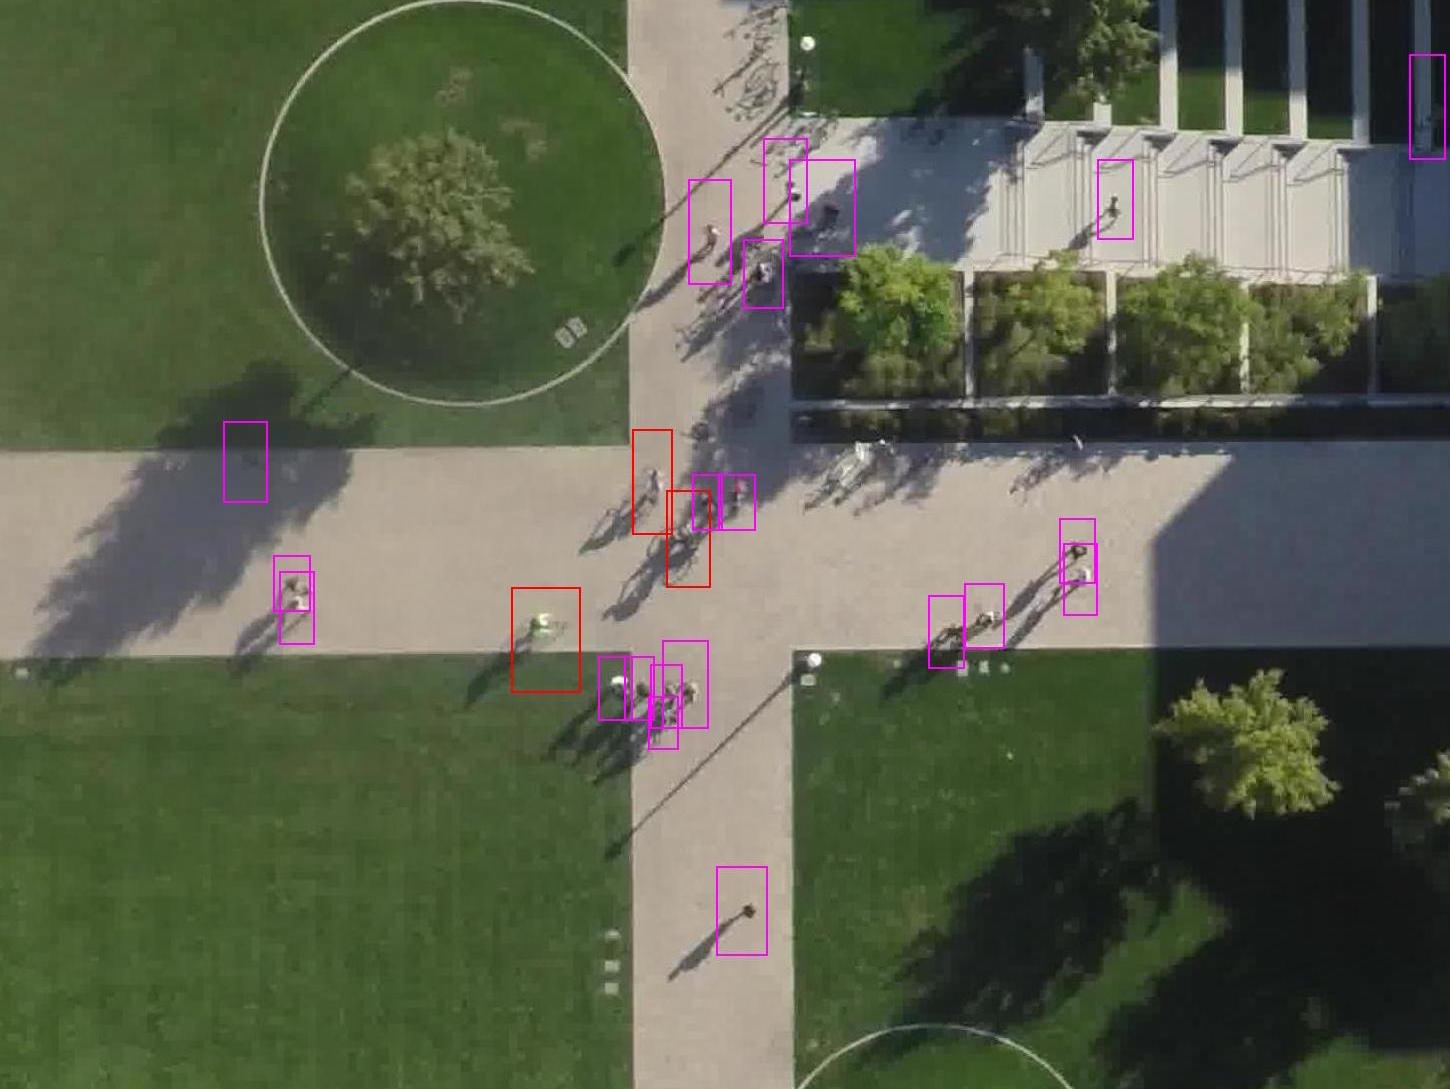
\includegraphics[width=0.42\linewidth]{3-sdd-example}
    \hfill
    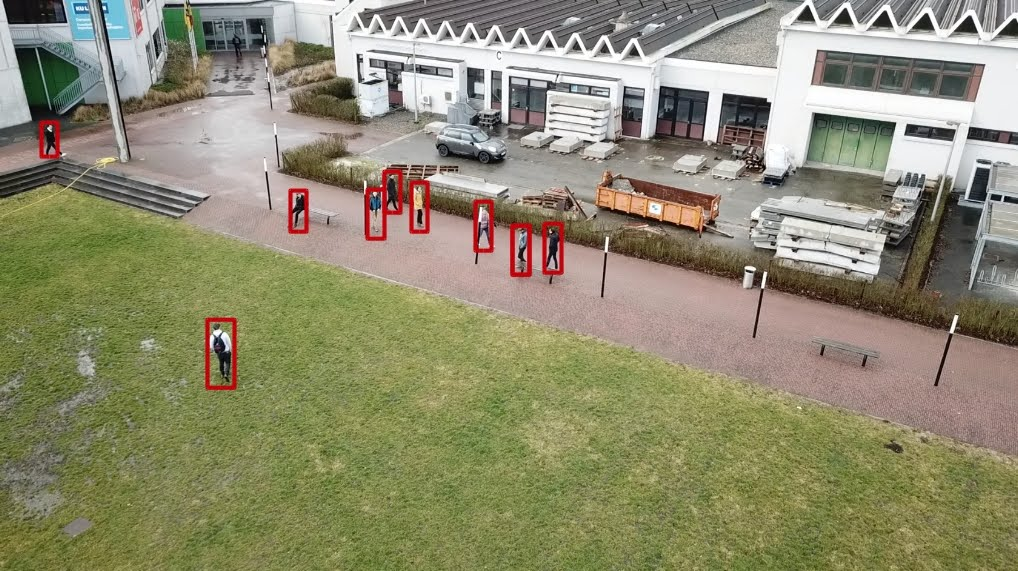
\includegraphics[width=0.56\linewidth]{3-visdrone-example}
    \caption{Примеры изображений SDD и VisDrone наборов данных} \label{sdd-visdrone-example}
\end{figure}


В силу специфичности решаемой задачи, пришлось самостоятельно формировать и организовывать сбор обучающей выборки с необходимыми нам фотографиями. Для решения этой задачи были привлечены добровольцы из различных ПСО, а также, разработаны методические материалы по сбору и разметке данных \cite{lib-lacmus-wiki-images}\cite{lib-lacmus-wiki-label}.

В результате был получен уникальный в своем роде набор данных, получивший в последствии название Lacmus Drone Dataset (LaDD) \cite{lib-ladd}. LaDD состоит из 1431 фотографии и имеет формат аннотирования Pascal VOC \cite{lib-pascal} с одним классом "Pedestrian" (пешеход). Dataset также является открытым и распространяется по лицензии GNU GPL v3. В его создании приняло участие множество ПСО из различных регионов России (Москва, Саратов, Ямал, Крым, Калининград и др). Таким образом, удалось достичь высокого разнообразия природных условий и, как следствие, и обучающей выборки. Ниже приведен пример фотографии:

\addimghere{3-ladd-example}{1}{Московская область, осень 2019, бурелом, лежачий на боку человек}{ladd-example}

\clearpage % Создание набора данных
\section{Архитектуры нейросетевых детекторов}\label{sect-4}

Различают несколько типов нейросетевых детекторов: One-stage и two-stage \cite{lib-detector-types}.

Two-stage -- более старый подход детекции. Он состоит из двух этапов. Сначала генерируются области, которые соответствуют искомым объектам. Ненужные области отсеиваются с помощью классификатора, например AlexNet \cite{lib-alexnet}. Такой подход является довольно точным, но не эффективен как по скорости, так и по памяти. Ярким примером такого подхода могут послужить такие архитектуры как: R-CNN и Faster R-CNN \cite{lib-rcnn}.

One-stage -- более быстрый и состоит из одного шага. Сначала изображение попадает в backbone -- базовую сверточную нейронную сеть. Сигналы из разных ее уровней пробрасываются в сеть трансформирующую признаки, а затем, производится классификация и детекция. Представителями этого подхода являются: SSD \cite{lib-ssd}, YOLO \cite{lib-yolo}, RetinaNet \cite{lib-retinanet}, TTFNet \cite{lib-ttfnet}.

\subsection{Выбор подходящего детектора}

В качестве кондидатов мною были выбраны лучшие архитектуры за последние 7 лет. Отбор производился на основе соремнований для задачи детекции MS COCO. Ниже приведен список этих типов СНС:
\begin{itemize}
    \item MobileNet-v3 + SSD -- one-stage детектор симейства SSD с MobileNet (v3) в качестве backbone;
    \item YOLO-v4 (Darknet-53) -- one-stage детектор симейства YOLO v4 с Darknet-53 в качестве backbone;
    \item EfficientDet-D3 -- one-stage детектор симейства Efficientdet с EfficientNet-B3 в качестве backbone;
    \item TTFNet-53 -- one-stage детектор симейства TTFNet с Darknet-53 в качестве backbone;
    \item RetinaNet (Resnet-50) -- one-stage детектор симейства RetinaNet с Resnet-50 в качестве backbone;
    \item Faster RCNN -- two-stage детектор симейства Faster RCNN.
\end{itemize}

Все перечисленные выше кондидаты были поставлены в одиноковые условия и обучались по одному алгоритму:
\begin{itemize}
    \item СНС инициализировалась со случайными весами;
    \item СНС обучалась на выборке MS COCO (100 эпох);
    \item Обученная на предыдущем шаге СНС дополнительно обучалась на LaDD и VisDrone (10 эпох).
\end{itemize}

Результаты эксперемента приведены в таблице \ref{leaderboard-table}.

\begin{table}[H]
    \caption{Сравнение различных архитектур детекторов}\label{leaderboard-table}
    \begin{tabular}{|p{4cm}|p{3cm}|p{3cm}|p{5cm}|}
    \hline
    {Тип} & {mAP (LaDD)} & {mAP (VisDrone)} & {Время обработки изображения (Tesla v100)} \\
    \hline
    MobileNet-v3 + SSD & 0.46 & 0.12 & 100 мс \\
    \hline
    YOLO-v4 (DarkNet-53) & 0.52 & 0.15 & 270 мс \\
    \hline
    EfficientDet-D3 & 0.66 & 0.23 & 400 мс \\
    \hline
    TTFNet-53 & 0.65 & 0.21 & 300 мс \\
    \hline
    RetinaNet (ResNet-50) & 0.71 & 0.25 & 300 мс \\
    \hline 
    Faster RCNN & 0.72 & 0.24 & 500 мс \\
    \hline
    \end{tabular}
  \end{table}

  Из эксперимента видно что по совокупности точности и скорости работы лучше всего справляется с детекцией RetinaNet. Также превосходтсво этой архитектуры подтверждает еще одно исследование. В нем сравнения СНС проводились на выборке Stenfird Drone Dataset (SDD) в которой содержится около 1 миллиона изображений снятых с БПЛА в кампусе Стенфордского Университета. Некоторые результаты этого исследования приведены в таблице \ref{leaderboard-table-sdd}.

  \begin{table}[H]
    \caption{Сравнение различных архитектур детекторов на выборке SDD}\label{leaderboard-table-sdd}
    \begin{tabular}{|p{7cm}|p{5cm}|}
    \hline
    {Тип} & {mAP (SDD)} \\
    \hline
    SSD (ResNet-50) & 0.80 \\
    \hline
    Faster RCNN (ResNet-50) & 0.83 \\
    \hline
    RetinaNet (Resnet-50) & 0.85 \\
    \hline
    \end{tabular}
  \end{table}

  Из вышеперечисленных исследований следует, что RetinaNet в сравнении с другими архитектурами обладает высокой точностью и скоростью работы и ее можно применять для решения задач детектирования объектов по снимкам с БПЛА.


\clearpage % Выбор архитектуры снс
\subsection{Устройство RetinaNet}\label{sect-5}

Архитектура RetinaNet, взятая за основу для моего исследования, состоит из ряда основных частей. Каждая из них выполняет определенную функцию:
\begin{itemize}
    \item backbone (или базовая сеть) -- необходима для извлечения тензора признаков (feature extraction) из входного изображения. В качестве нее может быть выбран один из нескольких вариантов СНС таких как: ResNet, EfficientNet, MobileNet и прочие;
    \item Feature Pyramid Network (FPN) -- пирамидальная СНС, необходима для трансформации признаков \cite{lib-fpn}. Она объединяет карты признаков приходящих как с верхних, так и с нижних уровней базовой СНС, так как первые обладают низкой обобщающей способностью (receptive field) при большей размерности, а последние -- наоборот;
    \item Classification Subnet Network (подсеть классификации) -- необходима для извлечения информации о классах. Классификация происходит для каждого уровня пирамиды, затем результаты фильтруются;
    \item Regression Subnet Network (подсеть регрессии) -- необходима для извлечения информации о положении объекта. Регрессия также происходит для каждого уровня пирамиды, затем результаты фильтруются;
    \item Блок пост обработки -- представляет собой набор алгоритмов для фильтрации предсказаний СНС. Как правило, здесь применяются такой алгоритм как NMS (Non Maximum Suppression) \cite{lib-nms}.
\end{itemize}

Ниже приведена общая архитектурная схема RetinaNet:

\addimghere{5-retinanet-architecture}{1}{Архитектурная схема RetinaNet}{retinanet-architecture}

Рассмотрим каждую из частей RetinaNet подробнее.

\subsection{Backbone}

Как говорилось выше, базовая сеть может быть реализована по разному. Так как от ее выходных признаков зависят предсказания остальных частей детектора -- необходимо выбрать наиболее подходящую архитектуру для backbone-СНС.

Для этого были проанализированы исследования последних лет. В качестве сравнительных характеристик были выбраны accuracy и времени работы, а в качестве обучающей выборки -- ImageNet. На изображение ниже приведены результаты исследований:

\addimghere{5-1-resnet-benchmark}{1}{Сравнение различных СНС на ImageNet 2020}{retinanet-architecture}

Представленная еще в 2015 году Microsoft Research архитектура ResNet \cite{lib-resnet} оказалась настолько удачной, что и по сей день периодически ставит рекорды в области распознавания изображений. Рассмотрим семейство архитектур ResNet подробнее.

Ее успех заключается в применении Residual блоков. С ростом числа слоев в нейронной сети все острее встает проблема паралича нейронной сети -- из-за обратного распространения ошибки градиент от слоя к слою постоянно уменьшается. В результате более глубокие слои перестают обучаться и как следствие качество распознавания падает:

\addimghere{5-1-cnn-back-propagation-paralysis}{0.8}{Увеличение колличества слоев дает ходший результат}{back-propagation-paralysis}

Основная идея ResNet заключается в том, чтобы ввести так называемое "соединение с пропусками" (Skip Connection), которое пропускает один или несколько уровней, как показано на рисунке ниже:

\addimghere{5-1-residual-block}{0.6}{Residual блок}{residual-block}

Благодаря Residual блокам, градиент не уменьшается, а слои СНС можно объединять в длинные последовательности, увеличивая как обобщающую способность, так и точность такой сети:

\addimghere{5-1-resnet-training-results}{1}{Кривые обучения ResNet (справа) с 18 и 34 слоями в сравнении с аналогичной СНС без residual обоков (слева)}{residual-block}
\subsection{Feature Pyramid Network} \label{sect-5-2}

FPN состоит из нескольких частей (рис. \ref{fpn-arch}): восходящей (bottom-up) и низходящей (top-down) пирамид, а также боковых соединений (lateral connections). Рассмотрим подробнее каджую часть.

\addimghere{5-2-fpn-arch}{0.8}{Архитектура FPN}{fpn-arch}

Восходяая пирамида -- есть некоторая последовательность светросных слоев, расзмерность которых уменьшается, извлекающяя признаки из входного изображения. В нашем случае это базовая сеть (ResNet50). Стоит отметить, что по с ростом уровней пирамиды увеличивается число информации, содержащиеся в каждос супер-пикселе сверточного слоя (receptive fild), но вместе с тем уменьшается размерность выходного тензора. 
Из-за этого факта bottom-up пирамида обладает уязвимостью -- важные призноки, особенно если обьект небольной, могут потерятся при перекрытии объекта (человек прикрыт травой) а конечные обьекты имеют размер в несколтко супер-пикселей (рис. \ref{fpn-distribution}). Как следистве СНС будет работать нестабильно, а колличество ошибок 1 и 2 рода возрастет. 

\addimghere{5-2-fpn-distribution}{0.6}{Внутреннее представление человека на одном из верхних уровней FPN}{fpn-distribution}

Некоторые пути решения этой проблемы будут рассмотрены в следующих разделах, а сконцентрируемся на устройстве FPN.

Низходящая пирамида -- напротив представляет собой полследовательность всерточных слоев размерность которых увеличивается по мере спуска сигнала. На каджом шаге размерность карт признаков возрастает в 2 раза, недостающие признаки выбираются методом ближайших соседей ((рис. \ref{fpn-top-down-knn})). Начальные уровни top-down пирамиды имеют такую же размерность что и верхние уровни bottom-up пирамиды, а размеры последних -- наоборот соответствуют первым уровням backbone-сети.

\addimghere{5-2-fpn-top-down-knn}{0.5}{Увеличение размерности признаков методом ближайшего соседа}{fpn-top-down-knn}

В добавок, между пирамидами в FPN существуют и боковые соединения. Благодаря ми, признаки соответствующих слоёв поэлементно складываются, причём карты из bottom-up пирамиды проходят через свёртку $1 \times 1$ (рис. \ref{fpn-connections}).

\addimghere{5-2-fpn-connections}{0.6}{Устройство боковых соеденений}{fpn-connections}

Уровни пизходящей пирамиды принято обозначать как $P_1, P_2, ..., P_n$, притом каждый $i$ уровень top-down пирамиды соответст сответствует $i$-му уровню bottom-up пирамиды $C_1, C_2, ..., C_n$. Кллличество $P$ уровней может быть меньше от колличества уровней $С$. Тогда уровни низходящей пирамиды могут быть сдвинуты на некоторый шаг. Так оригинальная FPN имеет конфигурацию с пятью уровнями $P_3...P_7$. На изображении ниже приведен пример FPN сети с кофигурацией $P_3...P_5$:

\addimghere{5-2-fpn-p3-p5}{0.8}{Архитектура FPN c $P_3...P_5$ уровнями}{5-2-fpn-p3-p5}
\subsection{Anchor boxes}

Анкерные или якорные рамки (anchor boxes) впервые были предложены в архитектуре Faster RCNN и затем получили свое распространение на многие современные архитектуры детекторов таких как YOLO или RetinaNet. 

Предположим, что СНС сворачивает исходное изображение до тензора размерности $3 \times 3$. Таким образом, в каждом супер-пикселе выходного тензора содержится информация о некоторой области исходного изображения. Тогда можно предположить размеры объекта попадающего в такой супер-пиксель (рис. \ref{anchor-boxes}). Эти размеры, их количество и ориентация и называются анкерными рамками (т.е. рамками "привязанными" к супер-пикселю). Для RetinaNet каждый супер-пиксель имеет анкоры с соотношениями сторон $2:1, 1:1, 1:2$ и размерами $2^0, 2^{\frac{1}{3}}, 2^{\frac{2}{3}}$ (и того 9 штук). При обучении модели для каждого объекта подбираются в наиболее подходящие анкоры. Если $IoU$ рамки больше 0.5, то она считается верной, а если меньше 0.4 -- ложной. В случаях когда $IoU \in [0.4 .. 05]$ anchor box будет проигнорирован для обучения.

\addimghere{5-3-anchor-boxes}{0.6}{Аnchor boxes}{anchor-boxes}
\subsection{Подсети классификации и регрессии}

Classification и regression subnet получают на вход признаки из нисходящей пирамиды FPN и выдают предсказания о классе и местоположении объекта. 

В подсети классификации сигнал сперва проходит через 4 сверточных слоя с размерностью $[3 \times 3]$, с 256 фильтрами и со стоящей после ReLU активацией. Таким образом, в каждом convolution слое формируется тензор размера $[h \times W \times 256]$ (256 карт признаков). Затем, сигнал снова проходит через сверточный слой $[3 \times 3]$, но уже с $K \times A$ фильтрами и сигмоидальной активацией. В результате, на выходе этой сети формируется вектор длиной $K \times A$, где $K$ -- количество разных классов (в нашем случае только один класс -- это Pedestrian), $A$ -- количество анкерных рамок. Подсеть для каждого анкера выдает one-hot вектор, где позиция числа 1 соответствует номеру класса для каждого анкера к которому модель отнесла объект.

В подсети регрессии первые 4 слоя эквивалентны соответствующим слоям в classification subnet. Затем, идет свертка,  $[3 \times 3]$ формирующая $4 \times A$ карт признаков. После чего, аналогично классификационной подсети, формируется вектор длинны $4 \times A$. Таким образом, подсеть позволяет уточнить 4-компонентный вектор координат анкера под реальный размер объекта: $(\Delta x_{min}, \Delta y_{min}, \Delta x_{max}, \Delta y_{max})$.
\subsection{Функция потерь}

Отметим, что функция потерь (loss function) складывается из двух компонент: ошибки регрессии и классификации (формула \ref{eq-1}).

\begin{equation}\label{eq-1}
    L = \lambda L_{reg}+L_{cls}
\end{equation}
где:
\begin{itemize}
    \item $L$ -- функция потерь RetinaNet;
    \item $L_{reg}$ -- ошибки регрессии;
    \item $L_{cls}$ -- ошибки классификации;
    \item $\lambda$ -- коэффициент усиления, определяющий соотношение между потерями.
\end{itemize}

Рассмотрим из чего складываются потери регрессии. Мы знаем, что каждому объекту ставится в соответствии анкерная рамка. Пусть $G$ -- целевой (ground truth) объект, а $A$ -- анкер. Тогда, сопоставив объекты и anchor box-ы получим $s$ пар: $(G_i, A_i), i=1..s$.

Заметим, что для каждого анкера regression subnet отдает вектор, показывающий разницу между границами якорной рамки и объекта: $(\delta x_{min}, \delta y_{min}, \delta x_{max}, \delta y_{max})$.  Подсчитав действительное расстояние между анкером и границами объекта  $(\Delta x_{min}, \Delta y_{min}, \Delta x_{max}, \Delta y_{max})$ и сравнив его с результатами работы подсети, вычислим потери регрессии:
$$
L_{reg} = \sum_{i, j} smooth_{L1}(\delta_{ij}-\Delta_{ij})
$$
где:
\begin{itemize}
    \item $\delta_{ij}$ -- прогнозируемое расстояние между anchor box-ом и границами объекта;
    \item $\Delta_{ij}$ -- реальное расстояние между anchor box-ом и границами объекта;
    \item $i \in {x, y},\ j \in {min, max}$;
    \item $smooth_{L1}(x) = \begin{cases}\frac{1}{2}x^2, & \mid x\mid < 0\\\mid x\mid - \frac{1}{2}, & x \geq 0\end{cases}$
\end{itemize}

Для потерь классификации используется функция Focal Loss \cite{lib-focal-loss}:
$$
L_{cls} = -\sum_{i=1}^K \alpha_i \cdot log(p_i)(1-p_i)^\gamma
$$
где:
\begin{itemize}
    \item $K$ -- количество классов;
    \item $p_i$ -- вероятность с которой класса $i$ был предсказан;
    \item $\gamma$ -- фокальный коэффициент;
    \item $\alpha_i$ -- коэффициент усиления класса $i$ (в нашем случае мы имеем только один класс и $\alpha$ = 1).
\end{itemize}

Данная функция есть усовершенствование функцией кросс-энтропии \cite{lib-focal-loss}, где от модели требуется высокая степень "уверенности" и влияние часто встречающихся классов возрастает. В Focal Loss это влияние, наоборот, снижается, а наибольший вклад при обучении весов RetinaNet оказывают редко встречающиеся объекты. Делается это за счёт множителя $(1-p_i)^\gamma$, а также параметров $\alpha_1$ и $\gamma \in(0, \infty)$. Графики функций focal и cross entropy представлены на рисунке ниже:

\addimghere{5-5-focal-loss}{0.8}{Графики focal loss и cross entropy}{focal-loss}

Стоит отметить, что во время обучения, большая часть объектов, обрабатываемых классификатором, является фоном, который является отдельным классом. Поэтому может возникнуть проблема, когда нейросеть обучится определять фон лучше, чем другие объекты. Такая несбалансированность очень характерно для решаемой задачи детектирования пропавших людей. По этому, в качестве функции потерь была выбрана Focal Loss.
\subsection{Пост-обработка}

Зачастую получается так, что СНС отдает на выходе несколько прогнозов указывающих на один и тот же объект. В этом случае такие предсказания следует отфильтровать, выбрав наилучшие (рис. \ref{nms}). Однако, при фильтрации стоит учитывать случай, когда на изображении два разных объекта одного класса могут находиться рядом, и их ограничивающие рамки могут пересекаться. Эта задача решается на этапе пост-обработки с помощью алгоритма Non-Maximum Suppression (NMS).

\addimghere{5-6-nms}{0.8}{Пример работы NMS}{nms}

На вход NMS принимает набор bounding box-ов для одного класса и порог, задающий величину максимального пересечения между ними. Ограничивающие рамки сортируются по уверенности (accuracy) и кладутся на стек. В первом цикле со стека берется очередная гипотеза. Затем, во вложенном цикле со стека берется вторая гипотеза. Если между двумя гипотезами IoU больше заданного порога, то вторая гипотеза отбрасывается. Алгоритм продолжает работу до тех пор пока не переберет все пары ограничивающих рамок.

Код алгоритма может выглядеть так:

\lstinputlisting[numbers=left]{inc/scripts/nms.py} % Описание retinanet
\section{Обучение RetinaNet и улучшение ее архитектуры}\label{sect-6}

Мною были предприняты несколько попыток обучения модели с использованием разных подходов, а также улучшения существующей архитектуры. Об этих экспериментах и об их результатах я расскажу в этом разделе.

\subsubsection{Эксперименты с размерностью входного тензора}

Важным гипер-параметром от которого зависит качество распознавания и скорость обработки является размер входного изображения. Очевидно, что с ростом размера изображения качество распознавания мелких объектов улучшается, однако, вместе с тем, увеличивается как потребление памяти, так и время работы алгоритма. Для проведения эксперимента была взята модель предобученная на выборке MS-COCO (100 эпох), а затем, она была доучена на LaDD (10 эпох) и выбрана лучшая модель. Результаты эксперимента приведены в таблице ниже:

\begin{table}[H]
    \caption{Эксперименты с размерами входного изображения}\label{image-size-table}
    \begin{tabular}{|p{7cm}|p{5cm}|}
        \hline
        {Размер картинки} & {mAP (LaDD)} \\
        \hline
        1333 $\times$ 800 & 0.71 \\
        \hline
        1500 $\times$ 2000 & 0.82 \\
        \hline
        4000 $\times$ 3000 & 0.84 \\
        \hline
    \end{tabular}
\end{table}

Как видно из результатов эксперимента, модель, обученная на оригинальных картинках (4000 $\times$ 3000), практически не опережает в качестве модель, обученную на снимках, уменьшенных в два раза, однако, сильно проигрывает в скорости работы (более чем в 4 раза) и в потреблении памяти (почти в 3 раза). Модель, обученная на картинках 1333 $\times$ 800, уже сильно отстает по точности. На рисунке ниже представлены фрагменты изображений с человеком для уменьшенного и оригинального снимка:

\addimghere{6-1-image-sizes}{0.8}{Фрагменты снимков с человеком для различных размеров}{image-sizes}

С этого момента и далее, при упоминании LaDD, на вход СНС будут подаваться картинки размера 1500 $\times$ 2000 точек.
\subsubsection{Предобучение на больших данных} \label{sect-6-2}

Важную часть в области глубокого обучения играют данные. Как правило, с ростом числа обучающей выборки растет и обобщающая способность нейронных сетей, а значит, и точность обработки изображений. За последние несколько лет наибольшего успеха в обучении СНС на больших объемах данных добилась команда исследователей из Facebook Research. В своем эксперименте \cite{lib-insta-net} ученые изучили насколько увеличение количества данных влияет на точность распознавания. Исследователи обучили сверточную нейронную сеть ResNet на 3,5 миллиардах изображений из социальной сети Instagram и сравнили ее с моделью обученной на ImageNet (1,2 миллиона изображений). Результат оказался впечатляющим -- полученная модель достигла качества 81.2\% accuracy на ImageNet, что является лучшем показателем в данном соревновании. 

\addimghere{6-2-instagram-resnet}{0.6}{Сравнение accuracy моделей с предобучением на 3,5 млрд. изображений и без}{instagram-resnet}

В связи с этим, я решил предобучить RetinaNet на большем по сравнению с MS COCO наборе данных и посмотреть на результаты. В качестве обучающей выборки был выбран OpenImagesDataset (OID) -- наибольший из доступных наборов данных для задачи детекции \cite{lib-iod}. Ниже приведено сравнение наборов данных OID и MS COCO:

\begin{table}[H]
    \caption{Характеристики наборов данных}\label{datasets}
    \begin{tabular}{|c|c|c|c|}
        \hline
        {Тип} & {Размер обучающей выборки} & {Число объектов} & {Число классов} \\
        \hline
        OID & 1.743 тыс. & 14.6 млн. & 600 \\
        \hline
        MS COCO & 200 тыс. & 1.5 млн. & 80 \\
        \hline
    \end{tabular}
\end{table}

За основу была взята модель, обученная на MS COCO, полученная ранее, и обучена уже описанным выше образом: сначала, СНС обучалась на OID наборе данных (100 эпох), затем, лучшая модель (mAP = 0.4326) была последовательно обучена на VisDrone и LaDD наборах данных (по 10 эпох). Сравнительная таблица с результатами полученных моделей приведена ниже.

\begin{table}[H]
    \caption{Сравнение моделей предобученных на MS COCO и OID}\label{leaderboard-2}
    \begin{tabular}{|p{7cm}|p{5cm}|}
        \hline
        {Выборка} & {mAP} \\
        \hline
        \multicolumn{2}{|c|}{С предобучением на MS COCO} \\
        \hline
        VisDrone & 0.25 \\
        \hline
        LaDD & 0.82 \\
        \hline
        \multicolumn{2}{|c|}{С предобучением на IOD} \\
        \hline
        VisDrone & 0.34 \\
        \hline
        LaDD & 0.87 \\
        \hline
    \end{tabular}
\end{table}

Как и ожидалось, увеличение количества данных привело к улучшению обобщающей способности СНС и уточнению скрытых представлений данных, благодаря чему, точность распознавания существенно возросла.
\subsection{Сдвиг FPN уровней} \label{sect-6-3}

Как говорилось в разделе \ref{sect-5-2}, FPN сеть имеет уязвимость, связанную с тем, что с ростом FPN уровней количество информации содержащейся в одном супер-пикселе (receptive field) увеличивается, при этом снижается размерность самой карты признаков. На практике это приводит к тому, что объекты малых размеров (люди, пни, коряги и т. д.) сворачиваются до нескольких супер-пикселей, из-за чего, СНС может легко перепутать человека и другой мелкий объект (например, пакет с мусором, или корягу). Это приводит к увеличению количества ложных срабатываний СНС и снижению эффективности алгоритма.

Первым и очевидным способом решить данную проблему является сдвиг FPN уровней вниз. Таким образом можно увеличить размерность карт признаков в FPN слоях. Для реализации этого подхода, программный код СНС был изменен таким образом, чтобы конфигурацию FPN пирамиды можно было задавать в конфигурационном файле, упрощая использование алгоритма. 

Так, в рамках эксперимента изначальная конфигурация FPN уровней ($P_3..P_7$) была изменена: все уровни сдвинулись на один вниз, а последний уровень был убран (для экономии вычислительных ресурсов). В результате получилась пирамида с конфигурацией $P_2..P_5$:

\addimghere{6-3-fpn-shift}{0.6}{Сдвиг уровней FPN}{5-2-fpn-shift}

Полученная модель была обучена аналогичным с приведенным в разделе \ref{sect-6-2} образом. Полученные в результате обучения результаты приведены в таблице ниже:

\begin{table}[H]
    \caption{Сравнение конфигураций FPN}\label{leaderboard-3}
    \begin{tabular}{|p{5cm}|p{5cm}|p{5cm}|}
        \hline
        {Тип модели} & {VisDrone, mAP} & {LaDD, mAP} \\
        \hline
        RetinaNet ($P_3..P_7$) & 0.34 & 0.87 \\
        \hline
        RetinaNet ($P_2..P_5$) & 0.42 & 0.90 \\
        \hline
    \end{tabular}
\end{table}

Из полученных результатов видно, что качество распознавания заметно улучшилось. Однако, вместе с увеличением размерностей и карт признаков, значительно возросло как время обработки изображения (в 3 раза), так и количество потребляемой памяти (более 4 Гб). Это затрудняет использование СНС на портативных компьютерах.
\subsection{Взвешенная FPN} \label{sect-wfpn}

В поисках более производительного решения, я проанализировал ряд научных статей, описывающих различные варианты модификаций FPN. Так, в одном из исследований \cite{lib-dfpn} FPN пирамида была углублена: более низкие уровни FPN были продублированы (рис. \ref{6-4-deep-fpn}). Такая конфигурации получила название Deep Feature Pyramid Network (DFPN). Основная идея DFPN заключается в том, что при повторении более низких уровней пирамиды увеличивается их вклад в предсказание СНС.

\addimghere{6-4-deep-fpn}{0.8}{Архитектурная схема DFPN}{6-4-deep-fpn}

Данное исследование натолкнуло меня на мысль о том, что различные уровни пирамиды признаков могут иметь для предсказания разное значение или вес. Как говорилось в разделе \ref{sect-5-2}, на каждом уровне нисходящей пирамиды сигнал складывается с соответствующим уровнем восходящей пирамиды, благодаря боковым соединениям. В оригинальной FPN эти сигналы имеют одинаковый, фиксированный вклад и результирующий сигнал равен их среднему значению, но это не оптимально. Действительно, на разных масштабах разные объекты могут представляться по разному. 

Для реализации этой идеи введем дополнительные усиливающие коэффициенты (веса) для каждого сигнала (рис. \ref{6-4-weight-fpn}) и будем вычислять результирующий сигнал с учетом этих коэффициентов $w^{j}_{i}$. Тогда признаки уровня $P_i$ будут вычисляться по следующей формуле:
$$
P_i = w^{C}_i \cdot C_i + w^{P}_i \cdot P_{i+1}
$$

Коэффициенты $w^{j}_{i}$ будем находить -- как и другие параметры СНС -- методом обратного распространения ошибки, нормализуя их в интервале $[0..1]$: $w^{j}_{i} = softmax(\Theta^{j}_{i})$. Во избежании больших значений обучаемых параметров $\Theta^{j}_{i}$ (и как следствие паралича СНС), будем применять к ним $L_2$ регуляризацию. Предлагаемая мной архитектура получила название Weight Feature Pyramid Network (WFPN).

\addimghere{6-4-weight-fpn}{0.4}{Схема Weight Feature Pyramid Network (WFPN)}{6-4-weight-fpn}

Для для проверки описанной выше гипотезы было произведено сравнение классической FPN с конфигурациями $P_3..P_7$ и $P_2..P_5$, DFPN конфигурации $P_3..P_7 + P_3..P_6 + ... + P_3$ и разработанной мной WFPN ($P_3..P_7$). Обучение моделей проводилось описанным в предыдущих разделах [\ref{sect-6-2}][\ref{sect-6-3}] способом. Размер входного изображения -- $2000\times1500$, обработка изображений проводилась на GPU nVidia Tesla V100.

\begin{table}[H]
    \caption{Сравнение конфигураций FPN}\label{leaderboard-full}
    \begin{tabular}{|c|c|c|c|}
        \hline
        {Тип модели} & {VisDrone, mAP} & {LaDD, mAP} & Время работы, мс \\
        \hline
        RetinaNet ($P_3..P_7$) & 0.34 & 0.87 & 400 \\
        \hline
        RetinaNet ($P_2..P_5$) & 0.42 & 0.90 & 1100 \\
        \hline
        RetinaNet-DFPN & 0.43 & 0.91 & 800 \\
        \hline
        RetinaNet-WFPN & 0.48 & 0.93 & 400 \\
        \hline
    \end{tabular}
\end{table}

Полученные результаты показывают, что Weight FPN не только демонстрирует лучшие результаты в задачи детектирования небольших объектов, но и работает с той же скоростью, что и классическая FPN. Также хочется отметить, что полученная архитектура является лучшей для задачи VisDrone (по метрике $mAP$). 

\addimghere{6-4-vis-drone-leaderboard}{1}{5 лучших решений задачи VisDrone}{6-4-vis-drone-leaderboard}

Полученные высокие результаты вполне можно объяснить и с точки зрения биологии: когда мы обронили что то маленькое и пытаемся это найти, мы фокусируемся на маленьких предметах и внимательно рассматриваем окружающее нас пространство. Введенные усиливающие коэффициенты в пирамиде признаков выполняют схожую функцию. Благодаря этому механизму, мы настраиваем внимание СНС, акцентируясь на мелких объектах, и находим баланс между размерностями карт признаков и их семантической грубиной (receptive field). К тому-же в WFPN веса непрерывны ($w^j_i\in[0..1]$), благодаря чему соотношение сигналов можно гибко изменять, за счет чего достигается преимущество предлагаемой архитектуры над DFPN.

\clearpage % Обучение модели
\section{Пользовательское программное обеспечние}

Запуск СНС как правило требует от пользователя поределенных навыков и умений, что сужает возможнсти сипользование СНС в ПСО. Для повышения удобства использования разработанного алгоритма машинного обучения было принято решение разработать пользовательское программное обеспечение (ПО). В процессе разработки ПО учитывались следубщие принципы:
\begin{itemize}
    \item простота -- приложение должно быть простым в использовании и утановке;
    \item платформонезависимость -- приложение должно работать на всех современных персональных компьютерах и операционных системах (linux, windows, osx);
    \item низкое потребление ресурсов -- прилодение должно быть эффетивным по памяти и по времмени;
    \item простота разработки -- прилодение должно обеспечивать высокую платформонезависимость программного кода для снижения стоимости разработки и поддержки.
\end{itemize}

Ниже будут описаны основные спекты процесса разработки прользовательского ПО и принципы построения его архитектуры а также причины выбора тех-или иных технологий для разработки.

\subsection{Оптимизация модели глубокого обучения} \label{sect-7-1}

Для возможности использования разработанной архитектуры WFPN на ПЭВМ и практического применения СНС в ПСО необходимо было как снизить ее требования к ресурсам, так и сократить время работы алгоритма или инференс (англ. inference) на портативных устройствах.

Для осуществления этих целей прибегают к следующим подходам:
\begin{itemize}
    \item Кванитизация -- это процесс уменьшения размера СНС в оперативной памяти компьютера. Уменьшение потребляемой памяти осуществляется путем уменьшения количества информации, необходимое для хранения одного параметра (веса) СНС. Так, например, изначально параметры модели имеют тип данных FP32. В процессе кванитизации тип данных может измениться на FP16 или даже INT8. Помимо снижения потребляемой памяти, кванитизация может привезти к уменьшению времени работы на различных устройствах. К примеру, на графических ускорителях nVidia модели с весами в формате FP16 могут выполняться до 2 раз быстрее, а кванитизация в INT8 ускоряет выполнение нейронных сетей на ARM устройствах;
    \item Объединение слоев СНС. Зачастую, некоторые слои СНС могут быть объеденины (например, свертка и ReLU активация), что приводит к увеличению производительности;
    \item Использование NPU (Neural Processor Unit) и TPU (Tensor Processor Unit) -- сопроцессоров, ускоряющих работу нейронных сетей;
    \item Использование аппаратно-ориентированных низкоуровневых библиотек, задействующих аппаратные возможности той, или иной платформы (например, AVX инструкции) для ускорения времени инференса.
\end{itemize}

Для практической реализации вышеупомянутых подходов мною были использованы следующие инструменты, библиотеки и устройства:

\begin{itemize}
    \item OneDNN (Tensorflow-oneDNN-2.3) - низкоуровневая библиотека обеспечивающая высокопроизводительное выполнение тензорных операций на x86 процессорах Intel и AMD \cite{lib-onednn};
    \item CUDA \cite{lib-cuda}, CuDNN \cite{lib-cudnn}, TensorRT \cite{lib-tensorrt} (Tensorflow-tensorrt-2.3) -- набор низкоуровневых библиотек и инструментов обиспечиваюие высокопроизводительное выполнение тензорных операций на графических ускорителях nVidia, а также объединение слоев и кванитизацию;
    \item Сопроцессоры Intel Movidius Myriad 2 \cite{lib-movidius} и Google Coral Edge TPU \cite{lib-coral} (рис. \ref{7-1-npus}) и соответствующие им наборы библиотек (OpenVINO \cite{lib-openvino} и Tensorflow-lite \cite{lib-tflite}).
\end{itemize}

Полученные результаты ускорения модели RetinaNet-WFPN приведены в таблице ниже:

\begin{table}[H]
    \caption{Оптимизация времени инференса RetinaNet-WFPN}\label{leaderboard-full}
    \begin{tabular}{|p{6cm}|c|c|p{2cm}|}
        \hline
        {Устройство} & {Библиотека} & {Формат} & {Время работы, мс} \\
        \hline
        Intel i7-9750H (6/12) @ 4.500GHz & Tensorflow-cpu-2.3 & FP32 & 1100 \\
        \hline
        Intel i7-9750H (6/12) @ 4.500GHz & Tensorflow-oneDNN-2.3 & FP16 & 800 \\
        \hline
        nVidia Quadro T1000 Mobile (4 Gb) & Tensorflow-gpu-2.3 & FP32 & 400 \\
        \hline
        nVidia Quadro T1000 Mobile (4 Gb) & Tensorflow-tensorrt-2.3 & FP16 & 300 \\
        \hline
        Intel i7-9750H (6/12) @ 4.500GHz + Intel Movidius Myriad 2 & OpenVINO & FP16 & 500 \\
        \hline
        Intel i7-9750H (6/12) @ 4.500GHz + Google Coral Edge TPU & Tensorflow-lite & INT8 & 240 \\
        \hline
    \end{tabular}
\end{table}

Из полученных результатов видно, что благодаря оптимизациям удалось уменьшить время работы алгоритма для CPU в 1.4 раза, для GPU в 1.3 раза. С применением сопроцессоров Intel Movidius Myriad 2 и Google Coral Edge TPU этот показатель составил 2.2 и 4.5 раза соответственно. В связи с этим, в дальнейшем для запуска СНС на ПЭВМ будем использовать библиотеки Tensorflow-oneDN для CPU, Tensorflow-tensorrt для GPU, а также, OpenVINO и Tensorflow-lite для сопроцессоров.

\addimghere{7-1-npus}{0.8}{Сопроцессоры Google Coral Edge TPU (сверху) и Intel Movidius Myriad 2 (снизу)}{7-1-npus}
\subsection{Архитектура пользовательского ПО}
Принимая во внимание, что пользовательское ПО должно работать на разных платформах (Windows, Linux, OSX), иметь единый, платформонезависимый код и при этом обладать низким потреблением ремурсов мною выби выбраны следующие технологии для разработки: язык программирования C\# и платформа dot net core, библиотеки ReactiveUI и AvaloniaUI для построения ПО с графичиским интерфейсом (GUI, Graphic User Interface). Опишем каждый из компонентов более подробно:

\begin{itemize}
    \item .NET core -- это кроссплатформенная управляемая программная среда с открытым исходным кодом позваляющая разработывать ПО для операционных систем Windows, Linux и macOS для архитектур ARM и x66;
    \item ReactiveUI -- набор библиотек для .NET, позволяющий разработывать приложения с приминением реактивной модели программирования и паттерна MVVM (Model-Viev-View Мodel). Данный подход позволяет разделить ПО на независимые модули: Viev (инкапсулирует в мебе представление ПО -- графический интерфейс), Model (содержит в себе бизнес-логику приложения), View Мodel (связывает Viev и Model предостваляя интерфейсу набор команд и привязок);
    \item AvaloniaUI -- набор библиотек для .NET позволяющий проектировать и отрисовывать GUI любой сложности для различных платформ. По сравнению с аналогами (Electron, GTK, QT, WPF) он обладает более низким потреблением ресурсов и высокой степенью интеграции с .NET core.
\end{itemize}

Пример интерфейса пользовательского ПО приведен на рисунке ниже:

\addimghere{7-2-gui}{0.8}{Главное окно программы}{7-2-gui}

\subsubsection{Запуск моделей глубокого обучения в .NET}

Как говорилось в разделе \ref{sect-7-1}, для высокопроизводительного инференса моделей глубокого обучения требуются низкоуровневые библиотеки. Эти библиотеки спроектированы для разного оборудования и имеют различные интерфейсы взаимодействия (API). Также, зачастую, для возможности использования того или иного оборудования необходима установка различных драйверов (например nVidia CUDA и CuDNN). В добавок, использование нейронных сетей часто требует наличие интерпретатора python и различных python зависимостей (например opencv-python, numpy и т д). Все это требует от пользователя дополнительных знаний и затрудняет установку ПО и использование СНС.

Для решения этой проблемы была разработана система модулей \cite{lib-plugins}. Основная идея заключается в том, что модель поставляется вместе с модулем, включающем в себя весь набор низкоуровневых библиотек, необходимых для работы того, или оного оборудования, а также программный код осуществляющий связку между С\slash С++ методами библиотек и .NET CLI (Common Language Infrastructure). Таким образом программный код C\# способен вызывать соответствующие низкоуровневые методы и осуществлять вычисления на том, или ином устройстве.

В свою очередь, каждый модуль предоставляет единообразный интерфейс взаимодействия -- $IObjectDetectionPlugin$. С помощью него, программа может узнать, на каких операционных системах способен работать модуль и с какими устройствами. Модули могут подключаться в программу независимо друг от друга. ПО анализирует платформу, на которой оно запущено, и предлагает установить пользователю модуль, обеспечивающий максимальную производительности на его оборудовании. Например, если у пользователя имеется GPU от nVidia -- программа предложит пользователю использовать модуль с CUDA, CuDNN и TensorRT. Все модули хранятся на удаленном сервере, а пользовательское ПО способно управлять ими по средствам менеджера модулей (система управления модулей схожа с менеджерами пакетов APT, PIP, NuGet). Исходный код интерфейсов приведен в приложении А.

Классификация платформ запуска моделей глубокого обучения представлена ниже:

\begin{itemize}
    \item Операционные системы:
    \begin{itemize}
        \item Linux
        \item Windows
        \item OSX
    \end{itemize}
    \item Вычислительные устройства:
    \begin{itemize}
        \item CPU
        \item GPU
        \begin{itemize}
            \item nVidia GPU
            \item AMD GPU
        \end{itemize}
        \item Сопроцессоры
        \begin{itemize}
            \item Google Edge TPU
            \item Intel Movidius NPU
        \end{itemize}
    \end{itemize}
\end{itemize}

Для работы с различными вычислительными устройствами используются различные наборы библиотек (так, например, для процессоров Intel и AMD используется oneDNN, для GPU от nVidia -- CUDA, CuDNN и TensorRT, а для GPU от AMD -- ROCm и DirectML). Применение той, или иной библиотеки может зависеть от операционной системы. С учетом этих особенностей мною были использованы следующие варианты конфигураций:

\addimghere{7-2-plotforms-tree}{0.8}{Дерево платформ и библиотек}{7-2-plotforms-tree}

Собранный модуль имеет следующую структуру: в корне модуля лежат .NET Core библиотеки, обеспечивающие вызов низкоуровневых компонентов и предоставляющие программе API для инициализации и вызова модуля, а в каталоге runtimes, находятся платформозависимые низкоуровневые компоненты (рис. \ref{7-2-plugin-tree}).

\addimghere{7-2-plugin-tree}{0.8}{Cтруктура модуля LаcmusRetineNetPlugin.CPU}{7-2-plugin-tree}

Благодаря предложенному подходу, пользователь может легко манипулировать модулями с моделями глубокого обучения в зависимости от его потребностей. Инкапсуляция в модулях низкоуровневых библиотек избавляет пользователя от ручной установки драйверов и компонентов, облегчая использование ПО. В добавок, такая система позволяет обновлять СНС без необходимости обновления самого ПО и его рекомпиляции, что упрощает процесс разработки и поддержки.

Общая схема архитектуры ПО приведена ниже:

\addimghere{7-2-app-arch}{0.8}{J,ofz fh[LacmusApp]}{7-2-app-arch}

Напоследок, хочется отметить, что данное ПО и все его компоненты (включая СНС) имеют открытый исходный код и распространяются свободно под лицензией GNU GPL v3 \cite{lib-lacmus} \cite{lib-lacmus-app}.


\clearpage % Разработка ПО
\section{Результаты применения ПО в поисково-спасательных отрядах}

Безусловно, главной целью рассматриваемого программного обеспечения является помощь спасателям в поисковых операциях и автоматизация процесса поиска пропавших людей. По этому, в процессе разработки ПО в приоритете всегда были удобство и простота его использования, а этап внедрения был очень важен.

Процесс внедрения ПО Lacmus начался еще на этапе его разработки и проходил постепенно и итеративно. Сперва была подготовлена первоначальная, пробная версия ПО, имеющая минимальный базовый функционал, которая была предложена ряду добровольцев из ПСО "Лиза Алерт". Затем, от пользователей была собрана обратная связь, учтены их пожелания, исправлены ошибки в работе программы, добавлены новые функции и уже обновленная версия ПО была предложена более широкому кругу людей. Данный процесс повторяется итеративно. 

Постепенно круг пользователей ПО Lacmus начал расширяться, программа начала внедряться в другие отряды и организации а география ее применения перестала ограничиваться Российской Федерацией. Для облегчения использования программы была создана электронная энциклопедия с методическими материалами \cite{lib-lacmus-wiki}, описывающими процесс установки на разные платформы, минимальные системные требования, графический интерфейс, требования к условиям съемки с помощью БПЛА, аспекты применения БПЛА, ответы на частозадаваемые вопросы. В добавок, был создан информационный канал с новостями проекта \cite{lib-lacmus-news} и форум технической поддержки \cite{lib-lacmus-chat}.

Все это облегчает внедрение и использование программы и способствует увеличению количества пользователей. На данный момент программное обеспечение используют такие организации и ПСО как: "Лиза Алерт", "Ангел", "Сова", "Запад", МЧС Российской Федерацией и Республики Беларусь. Все программное обеспечение имеет открытый исходный код и распространяется свободно и бесплатно \cite{lib-lacmus} \cite{lib-lacmus-app}.

В рамках внедрения ПО Lacmus некоторыми ПСО были проведены предварительные испытания его эффективности в природной среде в условиях, приближенных к реальной поисково-спасательной операции. В природной местности было размещено несколько статистов, выполняющих роль потерявшихся людей, затем, была произведена аэрофотосъемка локации с помощью БПЛА. Полученные снимки были проанализированы описанным в данном исследовании алгоритмом на месте проведения тестирования на ПЭВМ оператора БПЛА. Полученные результаты приведены в таблице:

\begin{table}[H]
    \caption{Результаты испытаний RetinaNet-WFPN различными ПСО}\label{leaderboard-full}
    \begin{tabular}{|p{2.8cm}|p{3cm}|p{3cm}|p{3cm}|p{3cm}|}
        \hline
        {ПСО} & {Количество сттистов} & {Количество найдеых статистов} & {Количество ложный сработываний} & {Количество снимеов} \\
        \hline
        Лиза Алерт (Москва) & 6 & 6 & 4 & 200 \\
        \hline
        Сова (Тула) & 5 & 5 & 2 & 100 \\
        \hline
        Ангел (Брест) & 4 & 4 & 5 & 80 \\
        \hline
    \end{tabular}
\end{table}

Как видно из таблицы, предлагаемая в данном исследовании СНС хорошо выполняет поставленную на нее задачу детектирования пропавших людей, а благодаря оптимизациям модели глубокого обучения и пользовательскому ПО -- СНС можно применять на месте проведения операции в лесу, что также ускоряет поиск. В добавок хочется сказать что ПСО "Ангел", Теплица Социальных технологий и другие информационные ресурсы и ПСО периодически освещают данное ПО в видео-отчетах \cite{lib-lacmus-pr1} \cite{lib-lacmus-pr2} и новостных статьях \cite{lib-lacmus-pr3} \cite{lib-lacmus-pr4} \cite{lib-lacmus-pr5}.

\clearpage % Внедрение ПО
\anonsection{Заключение}

В данной работе рассматривалась и решалась задача детектирования потерявшихся людей на аэрофотоснимках с БПЛА с помощью моделей машинного глубокого обучения. В ходе исследования были получены следующие результаты:
\begin{itemize}
    \item Проведен анализ поисково-спасательных операций, на основе которого, выявлены критерии съемки изображений и условия использования разрабатываемого алгоритма;
    \item Произведен сбор и подготовка обучающей выборки, необходимой для обучения нейросетевых математических моделей;
    \item Сделан сравнительный анализ различных архитектур СНС для решения поставленной задачи, в результате которого, была выбрана архитектура RetinaNet-ResNet50;
    \item Проведен разбор и анализ выбранной архитектуры;
    \item Проведено ряд исследований и экспериментов, направленных на повышения точности модели, в результате чего, была разработана новая архитектура СНС RetinaNet-ResNet50-WFPN (взвешенная FPN) достигшая точности детектирования mAP 93\%;
    \item Произведен ряд оптимизационных работ, направленных на уменьшение времени работы СНС на ПЭВМ, в результате чего, была достигнута скорость обработки изображения в 800 мс на центральном процессоре и 300 мс на графическом ускорителе;
    \item Разработано пользовательское программное обеспечение с графическим интерфейсом, способное работать на современных операционных системах Linux, Windows, OSX;
    \item Разработанное ПО было внедрено в поисково-спасательные отряды, собрана статистика его использования. 
\end{itemize}

Полученная модель глубокого бучения обладает довольно высоким показатель mAP как для решения поставленной задачи, так и для других задач детектирования мелких объектов. Архитектура RetinaNet-ResNet50-WFPN, также, является уникальной и содержит в себе научную новизну. Благодаря разработанному пользовательскому ПО, а также, применению различных оптимизаций, ускоряющих алгоритм, данную технологию можно успешно применять в поисково-спасательных операциях, снижая время поиска пропавшего человека. Это придает проекту высокую социальную значимость, ведь он может спасти не одну человеческую жизнь.

\clearpage % Заключение
\begingroup 
\renewcommand{\section}[2]{\anonsection{Библиографический список}}
\begin{thebibliography}{00}

\bibitem{lib-sidorenko}
    Васильева Р., Земнухова Л., Сидоренко А. и др.
    Сканирование горизонтов: роль информационных технологий в будущем гражданского общества /
    изд. <<Когито-Центрс>>, Москва 2020.

\bibitem{lib-deep-learning-book}
    Goodfellow I., Bengio Y., Courville A.
    The Deep Learning Book //
    MIT Press, 2016.

\bibitem{lib-lecun-cnn}
    Lecun Y., Bottou L.
    Gradient-based learning applied to document recognition //
    IEEE, 1998.

\bibitem{lib-perciptrone}
    Нейронные сети, перцептрон
    [Электронный ресурс] //
    Викиконспекты университета ИТМО
    URL: https://neerc.ifmo.ru/wiki/index.php?title=Нейронные\_сети,\_перцептрон
    (дата обращения: 01.05.2021)

\bibitem{lib-imagenet}
    Stanford  Vision  Lab,  Stanford  University,  Princeton  University.  ImageNet 
    [Электронный ресурс] //
    URL: http://www.image-net.org/
    (дата обращения: 01.05.2021)

\bibitem{lib-cnn}
    Сверточные нейронные сети
    [Электронный ресурс] //
    Викиконспекты университета ИТМО
    URL: https://neerc.ifmo.ru/wiki/index.php?title=Сверточные\_нейронные\_сети
    (дата обращения: 01.05.2021)

\bibitem{lib-detection-task}
    Sharma  P.  A  Practical  Guide  to  Object  Detection  using  the  Popular YOLO Framework – Part  III  (with  Python  codes)
    [Электронный ресурс] //
    URL: https://www.analyticsvidhya.com/blog/2018/12/practical-guide-object-detection-yolo-framewor-python/
    (дата обращения: 01.05.2021)

\bibitem{lib-ods-metrics}
    Лабинцев  Е.  Метрики в задачах машинного обучения
    [Электронный ресурс] //
    Блог компании Open Data Science
    URL: https://habr.com/ru/company/ods/blog/328372/
    (дата обращения: 01.05.2021)

\bibitem{lib-map-metric}
    Tan R. Breaking Down Mean Average Precision (mAP)
    [Электронный ресурс] //
    Towards data science
    URL: https://towardsdatascience.com/breaking-down-mean-average-precision-map-ae462f623a52
    (дата обращения: 01.05.2021)

\bibitem{lib-iou-metric}    
    Rosebrock A. Intersection over Union (IoU) for object detection
    [Электронный ресурс] //
    URL: https://towardsdatascience.com/breaking-down-mean-average-precision-map-ae462f623a52
    (дата обращения: 01.05.2021)

\bibitem{lib-sdd}     
    Stanford Drone Dataset
    [Электронный ресурс] //
    URL: https://cvgl.stanford.edu/projects/uav\_data/
    (дата обращения: 01.05.2021)

\bibitem{lib-visdrone}     
    VisDrone Object Detection
    [Электронный ресурс] //
    URL: http://aiskyeye.com/challenge\_2021/object-detection-2/
    (дата обращения: 01.05.2021)

\bibitem{lib-transfer-learning}  
    Sarkar D. A Comprehensive Hands-on Guide to Transfer Learning with Real-World Applications in Deep Learning
    [Электронный ресурс] //
    Towards data science
    URL: https://towardsdatascience.com/a-comprehensive-hands-on-guide-to-transfer-learning-with-real-world-applications-in-deep-learning-212bf3b2f27a
    (дата обращения: 01.05.2021)

\bibitem{lib-lacmus-wiki-images}
    Перевозчиков Г. Руководство по аэрофотосъемке для операторов БПЛА
    [Электронный ресурс] //
    Github Lacmus Wiki
    URL: https://github.com/lacmus-foundation/lacmus/wiki/Для-пользователей:-Руководство-по-аэрофотосъемке-для-операторов-БПЛА
    (дата обращения: 01.05.2021)

\bibitem{lib-lacmus-wiki-label}
    Перевозчиков Г. Разметка данных для обучения
    [Электронный ресурс] //
    Github Lacmus Wiki
    URL: https://github.com/lacmus-foundation/lacmus/wiki/Для-пользователей:-Разметка-данных-для-обучения
    (дата обращения: 01.05.2021)

\bibitem{lib-ladd}
    Lacmus Drone Dataset (LaDD)
    [Электронный ресурс] //
    Github
    URL: https://github.com/lacmus-foundation/ladd-utils
    (дата обращения: 01.05.2021)    

\bibitem{lib-pascal}
    The PASCAL VOC project
    [Электронный ресурс] //  
    URL: http://host.robots.ox.ac.uk/pascal/VOC/
    (дата обращения: 01.05.2021)

\bibitem{lib-detector-types}    
    Liu L. et al. 
    Deep Learning for Generic Object Detection: A Survey //
    Int. J. Comput. Vis. 2020. Vol. 128, No 2. P. 261–318.

\bibitem{lib-alexnet} 
    Krizhevsky, A., Sutskever, I.
    ImageNet Classification with Deep Convolutional Neural Networks //
    NIPS, pp. 1106–1114, 2012.

\bibitem{lib-rcnn}
    Gandhi R.
    R-CNN, Fast R-CNN, Faster R-CNN, YOLO — Object Detection Algorithms
    [Электронный ресурс] //
    Towards data science
    URL: https://towardsdatascience.com/r-cnn-fast-r-cnn-faster-r-cnn-yolo-object-detection-algorithms-36d53571365e
    (дата обращения: 01.05.2021)

\bibitem{lib-ssd}
    Wei L., Dragomir A.
    SSD: Single Shot MultiBox Detector //
    ArXiv 1512.02325v5, 2016.

\bibitem{lib-yolo}
    Bochkovskiy A., Chien-Yao Wang
    YOLOv4: Optimal Speed and Accuracy of Object Detection //
    ArXiv 2004.10934v1, 2020.

\bibitem{lib-retinanet}
    Tsung-Yi Lin, Goyal P., Girshick R., Kaiming He, Piotr Dollár
    Focal Loss for Dense Object Detection //
    ArXiv 1708.02002v2, 2018.

\bibitem{lib-ttfnet}
    Zili Liu, Tu Zheng, Guodong Xu, Zheng Yang, Haifeng Liu, Deng Cai
    Training-Time-Friendly Network for Real-Time Object Detection //
    ArXiv 1909.00700, 2019.

\bibitem{lib-coco}
    Common objects in context
    [Электронный ресурс] //
    URL: http://cocodataset.org/
    (дата обращения: 01.05.2021)

\bibitem{lib-mobilenet}
    Howard A., Sandler M., Chu G., Chen L., Chen B., Tan Z., Wang W., Hartwig A.
    Searching for MobileNetV3 //
    ArXiv 1905.02244v5, 2019.

\bibitem{lib-efficientdet}
    Tan M., Pang R., Quoc V.
    EfficientDet: Scalable and Efficient Object Detection //
    ArXiv 1911.09070v7, 2020.

\bibitem{lib-resnet}
    He K., Zhang X., Ren S., Sun J.
    Deep Residual Learning for Image Recognition //
    ArXiv 1512.03385v1, 2015.

\bibitem{lib-benchmark-sdd}
    Wang X. et al.
    Fast and Accurate, Convolutional Neural Network Based Approach for Object Detection from UAV //
    IECON 2018 - 44th Annual Conference of the IEEE Industrial Electronics Society. IEEE, 2018. P. 3171–3175.

\bibitem{lib-fpn}
    Lin T., Dollár P., Girshick R., He K., Hariharan B., Belongie S.
    Feature Pyramid Networks for Object Detection //
    ArXiv 1612.03144v2, 2017.

\bibitem{lib-nms}
    Sambasivarao K.
    Non-maximum Suppression (NMS)
    [Электронный ресурс] //
    Towards data science
    URL: https://towardsdatascience.com/non-maximum-suppression-nms
    (дата обращения: 01.05.2021)

\bibitem{lib-knn}   
    Rajakaruna A.
    Image Scaling Methods and MATLAB Implementations
    [Электронный ресурс] //
    URL: https://aditharajakaruna.wordpress.com/2013/07/12/image-scaling-methods-and-matlab-implementations/
    (дата обращения: 01.05.2021)

\bibitem{lib-focal-loss}
    What is Focal Loss and when should you use it?
    [Электронный ресурс] //
    URL: https://amaarora.github.io/2020/06/29/FocalLoss.html
    (дата обращения: 01.05.2021)

\bibitem{lib-insta-net}
    Mahajan D., Girshick R., Ramanathan V., He K., Paluri M., Li Y., Bharambe A.  
    Exploring the Limits ofWeakly Supervised Pretraining //
    ArXiv 1805.00932, 2018.

\bibitem{lib-iod}
    Open Images Dataset
    [Электронный ресурс] //
    URL: https://storage.googleapis.com/openimages/web/index.html
    (дата обращения: 01.05.2021)

\bibitem{lib-dfpn}
    Vaddi S., Jannesari A., Kumar C.
    Efficient Object Detection Model forReal-Time UAV Applications //
    ArXiv 1906.00786v1, 2019.

\bibitem{lib-onednn}
    oneAPI Deep Neural Network Library (oneDNN)
    [Электронный ресурс] //
    URL: https://github.com/oneapi-src/oneDNN
    (дата обращения: 01.05.2021)
    
\bibitem{lib-cuda}
    CUDA Toolkit Documentation
    [Электронный ресурс] //
    URL: https://docs.nvidia.com/cuda/index.html
    (дата обращения: 01.05.2021)

\bibitem{lib-cudnn}
    nVidia CuDNN Documentation
    [Электронный ресурс] //
    URL: https://docs.nvidia.com/deeplearning/cudnn/developer-guide/index.html
    (дата обращения: 01.05.2021)

\bibitem{lib-tensorrt}
    nVidia TensorRT Documentation
    [Электронный ресурс] //
    URL: https://docs.nvidia.com/deeplearning/tensorrt/developer-guide/index.html
    (дата обращения: 01.05.2021)

\bibitem{lib-movidius}
    Intel Neural Compute Stick 2
    [Электронный ресурс] //
    URL: https://software.intel.com/content/www/us/en/develop/hardware/neural-compute-stick.html
    (дата обращения: 01.05.2021)

\bibitem{lib-coral}
    Google Coral Edge TPU
    [Электронный ресурс] //
    URL: https://coral.ai/
    (дата обращения: 01.05.2021)

\bibitem{lib-openvino}
    OpenVINO Toolkit Overview
    [Электронный ресурс] //
    URL: https://docs.openvinotoolkit.org/latest/index.html
    (дата обращения: 01.05.2021)
 
\bibitem{lib-tflite}
    TensorFlow Lite
    [Электронный ресурс] //
    URL: https://www.tensorflow.org/lite/guide
    (дата обращения: 01.05.2021)

\bibitem{lib-dotnetcore}
    Перевозчиков Г. 
    Расставим точки над .NET Core и .NET Standard
    [Электронный ресурс] //
    gosha20777.github.io
    URL: https://gosha20777.github.io/code/2018/02/22/dotnetcore/
    (дата обращения: 01.05.2021)

\bibitem{lib-reactiveui}
    ReactiveUI
    [Электронный ресурс] //
    URL: https://www.reactiveui.net/
    (дата обращения: 01.05.2021)    

\bibitem{lib-avaloniaui}
    AvaloniaUI
    [Электронный ресурс] //
    URL: https://avaloniaui.net/
    (дата обращения: 01.05.2021)

\bibitem{lib-mvvm}
    MVVM: полное понимание (+WPF) Часть 1
    [Электронный ресурс] //
    Habr
    URL: https://habr.com/ru/post/338518/
    (дата обращения: 01.05.2021)
    
\bibitem{lib-plugins}
    Перевозчиков Г. 
    Система плагинов: как завезти нейронные сети в dotnet
    [Электронный ресурс] //
    gosha20777.github.io
    URL: https://gosha20777.github.io/tutorial/2020/03/22/plugin-system/
    (дата обращения: 01.05.2021)
    
\bibitem{lib-lacmus}
    Lacmus Neural Network
    [Электронный ресурс] //
    URL: https://github.com/lacmus-foundation/lacmus
    (дата обращения: 01.05.2021)

\bibitem{lib-lacmus-app}
    Lacmus Application
    [Электронный ресурс] //
    URL: https://github.com/lacmus-foundation/lacmus-app
    (дата обращения: 01.05.2021)

\bibitem{lib-lacmus-wiki}
    Lacmus Wiki
    [Электронный ресурс] //
    URL: https://github.com/lacmus-foundation/lacmus/wiki/
    (дата обращения: 01.05.2021)    
    
\bibitem{lib-lacmus-news}
    Lacmus News
    [Электронный ресурс] //
    URL: https://t.me/lacmus\_news
    (дата обращения: 01.05.2021) 
    
\bibitem{lib-lacmus-chat}
    Lacmus Forum
    [Электронный ресурс] //
    URL: https://t.me/found\_lacmus
    (дата обращения: 01.05.2021)

\bibitem{lib-lacmus-pr1}
    ПСО "Ангел", г. Брест -- тестирование ПО Lacmus
    [Электронный ресурс] //
    URL: https://www.youtube.com/watch?v=HIf5LREOz-o
    (дата обращения: 01.05.2021)
    
\bibitem{lib-lacmus-pr2}
    Лиза Алерт, Лакмус и сервера в воде
    [Электронный ресурс] //
    URL: https://www.youtube.com/watch?v=4QfOBTHEgJU
    (дата обращения: 01.05.2021)

\bibitem{lib-lacmus-pr3}
    Лакмус. Нейросети находят пропавших людей
    [Электронный ресурс] //
    URL: https://vc.ru/u/619734-lacmus-foundation/167997-lakmus-neyroseti-nahodyat-propavshih-lyudey
    (дата обращения: 01.05.2021)
    
\bibitem{lib-lacmus-pr4}
    Нейросеть поможет найти потерявшихся людей
    [Электронный ресурс] //
    URL: https://www.if24.ru/nejroset-liza-alert/
    (дата обращения: 01.05.2021)

\bibitem{lib-lacmus-pr5}
    IT-волонтерство: как нейросеть ищет новороссийцев и не только в лесу
    [Электронный ресурс] //
    URL: https://bloknot-novorossiysk.ru/news/it-volonterstvo-kak-neyroset-ishchet-novorossiytse-1296563?fbclid=IwAR3ESOUSx7nrzb9b3xsbo7-U0R\_iEbPMqLjf3Q6a6Ohxh1A3BwW04Cr77Ag
    (дата обращения: 01.05.2021)

\end{thebibliography}
\endgroup

\clearpage % Библиографический список

% Приложения
\vspace*{\fill}
\centering{\uppercase{Приложение}}
\vspace*{\fill}

\clearpage

\appsection{Приложение А}
\centering{\uppercase{Исходный код интерфейсов системы модулей и модуля LacmusRetinanetPlugin.DirectML}}
\vspace{\baselineskip}

\lstinputlisting[numbers=left]{inc/scripts/lacmus-plugins/LacmusPlugin/IObjectDetectionPlugin.cs}

\lstinputlisting[numbers=left]{inc/scripts/lacmus-plugins/LacmusPlugin/IObjectDetectionModel.cs}

\lstinputlisting[numbers=left]{inc/scripts/lacmus-plugins/LacmusPlugin/IObject.cs}

\lstinputlisting[numbers=left]{inc/scripts/lacmus-plugins/LacmusPlugin/Version.cs}

\lstinputlisting[numbers=left]{inc/scripts/lacmus-plugins/LacmusPlugin/Enums/InferenceType.cs}

\lstinputlisting[numbers=left]{inc/scripts/lacmus-plugins/LacmusPlugin/Enums/OperatingSystem.cs}

\lstinputlisting[numbers=left]{inc/scripts/lacmus-plugins/LacmusRetinanetPlugin.DirectML/Model.cs}

\lstinputlisting[numbers=left]{inc/scripts/lacmus-plugins/LacmusRetinanetPlugin.DirectML/Plugin.cs}

\clearpage % Исходный код Plugin system
%\input{inc/b-app} % Руководство пользователя

\end{document}
%%% Конец документа